\documentclass[10pt,twocolumn,a4paper]{article}

\usepackage[top=20mm,bottom=20mm,left=15mm,right=15mm,columnsep=6mm]{geometry}
\usepackage{iftex}
\ifPDFTeX
  \usepackage[utf8]{inputenc}
  \usepackage[T5]{fontenc}
\else
  \usepackage{fontspec}
\fi
\usepackage[vietnamese]{babel}
\usepackage{booktabs}
\usepackage{tabularx}
\usepackage{amsmath}
\usepackage{amssymb}
\usepackage{graphicx}
\usepackage[hidelinks]{hyperref}
\usepackage{natbib}
\usepackage{placeins}
\usepackage{dblfloatfix}
\usepackage{microtype}

\setlength{\parindent}{0pt}
\setlength{\parskip}{5pt}
\renewcommand{\arraystretch}{1.12}
\newcommand{\verified}{\textbf{[đã kiểm chứng]}}

\title{\textbf{Học Tăng cường Q-Learning Đa mục tiêu theo\\Không gian--Thời gian cho Điều phối Công bằng}\\
\large Nghiên cứu Tái lập Định tính Độc lập trên Lát cắt Thời gian Taxi NYC 2013}
\author{
  \textbf{Dương Đức Cường}$^*$ \qquad \textbf{Nguyễn Huy Hoàng}$^\dagger$ \\[0.5em]
  \small Thực tập Nghiên cứu AI, Nhóm Điều phối Gọi xe (Ride Allocation Group) \\[0.3em]
  \small $^*$Tác giả chính; thiết kế và thực thi nghiên cứu tái lập, phân tích và thực nghiệm. \\
  \small $^\dagger$Mentor và tác giả liên hệ.
}
\date{\small Ảnh chụp tiến độ: 20 Tháng 8, 2026}

\begin{document}
\makeatletter
\twocolumn[
  \begin{@twocolumnfalse}
    \maketitle
    \begin{abstract}
    Chúng tôi thực hiện tái lập độc lập, xây dựng lại từ đầu, các XU HƯỚNG định
    tính được báo cáo bởi \citet{fairdispatch2024} cho một chính sách điều phối
    gọi xe có ràng buộc công bằng và dự báo nhu cầu (MOMAQL), \emph{không phải}
    tái lập số liệu chính xác -- paper gốc không cung cấp đủ chi tiết triển khai
    để đó là mục tiêu có ý nghĩa. Thử nghiệm trên lát cắt thời gian taxi NYC 2013
    thực tế (912.375 cuốc huấn luyện / 195.508 cuốc kiểm định, 200 tài xế mô
    phỏng), so sánh 5 chính sách điều phối, chạy bóc tách 3 nhánh, quét đánh đổi
    hiệu quả/công bằng, và -- theo đúng tuyên bố trung tâm của paper -- theo dõi
    công bằng khi khung thời gian đánh giá tăng từ 1 đến 7 ngày. Chúng tôi tái
    lập sạch các tuyên bố về đánh đổi và vượt trội baseline; các tuyên bố về
    horizon dài và no-fairness chỉ tái lập một phần, được định lượng và công bố
    rõ ràng thay vì làm tròn thành "đã tái lập hoàn toàn." Toàn bộ số liệu ở đây
    là kết quả mô phỏng thực.
    \end{abstract}
    \vspace{1.5em}
  \end{@twocolumnfalse}
]
\makeatother

\section{Chúng Tôi Đang Tái Lập Cái Gì}
\citet{fairdispatch2024} tuyên bố nhiều hơn "phương pháp của chúng tôi vượt
baseline." Bảng~\ref{tab:claims} nêu các tuyên bố cụ thể, kiểm chứng được mà
chúng tôi kiểm tra, mỗi cái đối chiếu với 1 bằng chứng cụ thể của mình.

\begin{table}[t]
\centering
\caption{Các tuyên bố được kiểm tra và kết luận trong nghiên cứu tái lập này.}
\label{tab:claims}
\footnotesize
\begin{tabularx}{\linewidth}{@{}p{0.06\linewidth}X p{0.18\linewidth}@{}}
\toprule
ID & Tuyên bố & Kết luận \\
\midrule
C1 & Utility và công bằng đánh đổi lẫn nhau & Đã tái lập \\
C2 & Phương pháp đề xuất vượt trội \emph{baseline đã điều chỉnh} trong bối cảnh này & Đã tái lập (có phạm vi) \\
C3 & Phương pháp RL ổn định hơn khi horizon tăng & Tái lập một phần \\
C4 & Dự báo giúp công bằng dài hạn, có thể tốn ngắn hạn & Tái lập một phần \\
C5 & Bóc tách: thành phần nhìn trước giúp cả utility+công bằng so với bị triệt tiêu & Đã tái lập \\
C6 & Bỏ công bằng tối đa hóa utility, bất bình đẳng bùng nổ & Tái lập một phần / Mâu thuẫn \\
\bottomrule
\end{tabularx}
\end{table}

\section{Bài Toán, Theo Ngôn Ngữ Của Chúng Tôi}
Bộ điều khiển tối đa hóa $\text{utility} - \lambda\cdot\text{bất công bằng}$
trên một khung thời gian dài, trong đó dự báo nhu cầu giúp hệ thống không tối
ưu công bằng một cách cận thị theo từng cửa sổ. Cụ thể trong triển khai của
chúng tôi: trạng thái là cặp (tài xế, yêu cầu) khả thi được chấm điểm ở mỗi
cửa sổ điều phối 60 giây; hành động là một phép gán chung giải 1 lần mỗi cửa
sổ (thuật toán Hungarian, từ chối ghép là lựa chọn thực sự); phần thưởng là
cước phí ròng trừ chi phí chạy rỗng; công bằng đo trên thu nhập
\emph{tích lũy} của tài xế, không phải phần thưởng tức thời, nên chính sách
không thể "lách" công bằng bằng cách luân phiên thiệt hại ai đó theo từng cửa
sổ; dài hạn khác ngắn hạn ở số ngày thu nhập tích lũy mà chỉ số công bằng
được tính trên đó -- chính xác là điều Mục~\ref{sec:horizon} kiểm tra.

\section{Nguồn gốc Dữ liệu}
Mẫu Bernoulli thực từ bộ dữ liệu NYC TLC 2013 đã làm sạch của dự án gốc
(tháng Development 1--8), lọc theo \texttt{manhattan\_both=true} và
\texttt{quality\_flag\_bitset=0}. Bảng~\ref{tab:lineage} cho số dòng còn lại
ở mỗi giai đoạn sau khi làm sạch upstream của chính dự án này (bộ lọc
manhattan/chất lượng do pipeline gốc của dự án áp dụng, tái sử dụng ở đây,
không tự làm lại).

\begin{table}[h!]
\centering
\caption{Nguồn gốc dữ liệu (số dòng thực tế).}
\label{tab:lineage}
\footnotesize
\begin{tabular}{@{}lr@{}}
\toprule
Giai đoạn & Số dòng \\
\midrule
NYC TLC 2013 thô (tất cả tháng) & 171.816.340 \\
Tập Development (tháng 1--8) & 115.707.941 \\
Lọc Manhattan + chất lượng, mẫu 1,3tr & 1.303.393 \\
Huấn luyện (chia theo thời gian) & 912.375 \\
Kiểm định & 195.508 \\
Kiểm thử & 195.510 \\
\bottomrule
\end{tabular}
\end{table}

\section{Paper so với Bản Tái Lập}
Bảng~\ref{tab:papervsrepl} nêu rõ mọi sai khác -- theo tinh thần
\citet{fairdispatch2024}, công bố rõ mới là điểm mạnh, không phải điểm yếu.

\begin{table*}[t]
\centering
\caption{So sánh từng thành phần.}
\label{tab:papervsrepl}
\footnotesize
\begin{tabularx}{\textwidth}{@{}lXXl@{}}
\toprule
Thành phần & Paper & Bản tái lập & Trạng thái \\
\midrule
Dữ liệu & NYC Taxi, 3--4/2016 & NYC TLC 2013, tháng 1--8 & Sai khác (năm) \\
Vùng & Manhattan & Manhattan (\texttt{manhattan\_both}) & Khớp \\
Số tài xế & Không nêu rõ & 200 & Giả định \\
Biểu diễn không gian & Gộp node đồ thị vị trí & 67 zone TLC & Xấp xỉ \\
Mô hình dự báo & MLP 3 lớp, OD-pair$\times$giờ & $Q$(vùng,giờ) dạng bảng, TD(0) trực tuyến & Sửa đổi (xem \S\ref{sec:terminology}) \\
$\lambda$ (trọng số công bằng) & 1 & 0,5 mặc định (quét 0--1) & Sai khác \\
$\omega$ (hệ số scale) & 0,6 & Không dùng; dùng chuẩn hóa fairness tương đối & Sửa đổi \\
$\gamma$ (discount) & 0,9 & 0,9 & Khớp \\
Baseline & Greedy, REASSIGN, LAF, Balance-RP & Greedy, Nearest, LAF, Exact REASSIGN & Trùng 1 phần \\
Luật ghép cặp & $\sum_v I_{rv}\le1$ (cho phép từ chối) & Hungarian đệm dummy, decline=0 & Khớp (đã verify với text paper) \\
Horizon đánh giá & 1--7 ngày & 1--7 ngày + toàn bộ 37 ngày & Khớp (mở rộng) \\
\bottomrule
\end{tabularx}
\end{table*}

\subsection{Thuật ngữ Chuẩn hóa}
\label{sec:terminology}
\textbf{$Q(\text{vùng},\text{giờ})$ là bộ ước lượng giá trị RL, KHÔNG phải
bộ dự báo nhu cầu.} Học qua bootstrap Bellman TD(0)
($Q(P,h)\leftarrow Q(P,h)+\alpha[\text{reward}+\gamma Q(D,h')-Q(P,h)]$,
reward $=$ cước phí $-$ chạy rỗng), đại lượng nó học là \emph{doanh thu
ròng kỳ vọng chiết khấu tương lai (USD) khi đứng ở 1 vùng vào 1 giờ} -- một
hàm giá trị theo nghĩa RL, khác về bản chất so với MLP của paper, vốn dự
báo \emph{số lượng yêu cầu} $\hat D_{ij,t}$ theo từng cặp điểm đón--trả mỗi
giờ. Chúng tôi KHÔNG gọi $Q$ là bản thay thế cho mô-đun dự báo đó, và không
gọi nó là mạng nơ-ron. Tương quan báo cáo giữa $Q$ và số lượng đón khách
thực tế tương lai ($r=+0,51$, \S\ref{sec:bug}) là \emph{chẩn đoán khả dĩ}
(vùng giá trị cao có xu hướng cũng có nhiều nhu cầu tương lai không?),
KHÔNG phải tuyên bố $Q$ \emph{là} một ước lượng nhu cầu -- đây là 2 đại
lượng khác nhau, tình cờ có thể đối chiếu được với nhau.
\textbf{Khung nghiên cứu:} đây là \emph{tái lập định tính độc lập trên lát
cắt thời gian thay thế} (2013 so với 2016 của paper), không phải tái lập
trên đúng năm dữ liệu của paper -- cung cấp bằng chứng rằng hành vi định
tính có thể quan sát được dưới 1 lát cắt thời gian khác, không phải bằng
chứng về khả năng tổng quát hóa qua các năm.
\textbf{Chuẩn hóa hàm mục tiêu:} điểm số của chúng tôi kết hợp cước
phí/chạy rỗng (USD) và khoảng cách công bằng \emph{tương đối} (phân số thu
nhập trung bình $\times$ cước phí cuốc này, tự nó cũng là USD) -- một hàm
mục tiêu ĐÃ SỬA ĐỔI, không phải dạng
$(1-\lambda)\cdot\text{utility}-\lambda\omega\cdot\text{Var}(U)$ của
chính paper. 2 $\lambda$ KHÔNG tương đương trực tiếp: $\lambda=1$ của
chúng tôi là cực thuần-công-bằng của 1 công thức khác, không phải giới hạn
của $\lambda=1$ mà paper báo cáo. Chúng tôi không tuyên bố tương ứng toán
học giữa 2 công thức.

\subsection{Định nghĩa Utility và Công bằng (A8, A9)}
\textbf{A8 -- utility.} Xác nhận trực tiếp từ \texttt{src/simulator.py}:
\texttt{net = fare\_amount - eta*0.0025} (cước phí USD thực trừ chi phí
thời gian chạy rỗng), tích lũy theo tài xế. Đây là chỉ số doanh thu thực.
Phần thưởng tức thời của paper được mô tả là hàm lợi ích/chi phí địa lý gắn
với điểm đón, điểm trả và vị trí tài xế -- CHƯA xác nhận là cùng đại
lượng. Do đó chúng tôi báo cáo xu hướng và so sánh tương đối trong bối
cảnh của mình, KHÔNG so sánh giá trị utility tuyệt đối với Bảng 1/2 của
paper như thể cùng đơn vị.

\textbf{A9 -- công bằng.} Gini là chỉ số chính xuyên suốt báo cáo. Chỉ số
chính của paper là $\text{Var}(U_1,\ldots,U_n)$ (và biến thể chuẩn hóa
$\sigma(U)/\bar U$); \texttt{common\_loader.py} có hàm
\texttt{variance}/\texttt{std}/\texttt{coefficient\_of\_variation}, giờ đã
báo cáo song song Gini cho R1 (Bảng~\ref{tab:r1}), R2 (Bảng~\ref{tab:r2}),
và Pareto sweep (\texttt{pareto\_frontier\_summary.csv}), tất cả đã chạy
lại để lưu thu nhập thô từng tài xế. Vẫn dùng Gini làm chỉ số dẫn dắt thay
vì CV, vì CV không ổn định khi utility trung bình gần 0
(\S\ref{sec:terminology}).

\section{Độ Trung thực của Baseline}
\begin{table}[t]
\centering
\caption{Mỗi baseline liên hệ thế nào với nguồn gốc của nó.}
\label{tab:baselines}
\footnotesize
\begin{tabularx}{\linewidth}{@{}p{0.12\linewidth}p{0.20\linewidth}p{0.09\linewidth}X@{}}
\toprule
Baseline & Nguồn & Exact/Approx & Sửa đổi \\
\midrule
Greedy & Paper & Exact & Không \\
Nearest & Không có trong paper & --- & Tự thêm, không phải baseline của paper \\
LAF & \citet{suhr2019} (ý tưởng gốc)$^\ddagger$ & Approx & Dùng khoảng cách công bằng tương đối, không phải chênh lệch thu nhập thô \\
Exact REASSIGN & \citet{lesmana2019} & Approx & Hungarian M-to-N theo lô, cho phép từ chối \\
MOMAQL & Paper & Approx & Bộ ước lượng giá trị RL dạng bảng, không phải MLP của paper (\S\ref{sec:terminology}) \\
\bottomrule
\end{tabularx}
\end{table}

\noindent\footnotesize$^\ddagger$Nguồn gốc ban đầu của LAF ("Shi et al.")
không xác minh được là một công bố thật, tìm được -- chúng tôi trích dẫn
\citet{suhr2019} thay thế, đây là công trình thật, kiểm chứng được, gần
nhất với cùng ý tưởng gốc (phân bổ công bằng thu nhập tài xế qua nhiều lần
ghép cặp thay vì ép công bằng từng lần). Không tuyên bố LAF là bản triển
khai trực tiếp thuật toán cụ thể của paper đó.
\normalsize

\section{Phương pháp}
\verified{} Pipeline đã thực thi: cuốc xe thực $\to$ chia theo thời gian
$\to$ mô phỏng theo lô cửa sổ 60s $\to$ ghép cặp Hungarian M-to-N $\to$ 5
chính sách (gồm MOMAQL) $\to$ chỉ số utility/Gini/phương sai.

Điểm MOMAQL: $s = (1-\lambda)[f - c\eta + \gamma Q(D,h')] + \lambda\big[\tfrac{\bar I - I_d}{\bar I}\big]f$.
Cập nhật $Q$ (Bellman TD(0)): $Q(P,h) \leftarrow Q(P,h) + \alpha[f - c\eta +
\gamma Q(D,h') - Q(P,h)]$, $(P,h)$ vùng/giờ đón, $(D,h')$ vùng/giờ trả, cả
hai đều là giờ thực tế tuyệt đối (epoch, không phải tương đối theo từng tập
-- các tập khác nhau có mốc thời gian khác nhau). $\alpha=0,1$, $\gamma=0,9$.

\section{Kết quả}

\subsection{R1: So sánh Cơ sở}
\begin{table}[h!]
\centering
\caption{195.508 yêu cầu kiểm định thực, 200 tài xế, trung bình 5 seed.}
\label{tab:r1}
\footnotesize
\begin{tabular}{@{}lrrrr@{}}
\toprule
Chính sách & Utility (\$) & Gini & PS ($\times10^6$) & Số chuyến \\
\midrule
MOMAQL & 1.422.441 & 0,204 & 8,35 & 152.380 \\
Greedy & 1.001.551 & 0,531 & 30,50 & 104.816 \\
Nearest & 789.444 & 0,430 & 9,94 & 86.370 \\
LAF & 766.265 & 0,002 & 0,0007 & 80.431 \\
Exact REASSIGN & 648.160 & 0,417 & 6,33 & 63.401 \\
\bottomrule
\end{tabular}
\end{table}
\footnotesize PS = Phương sai (Variance).\normalsize
\begin{figure}[t]
\centering
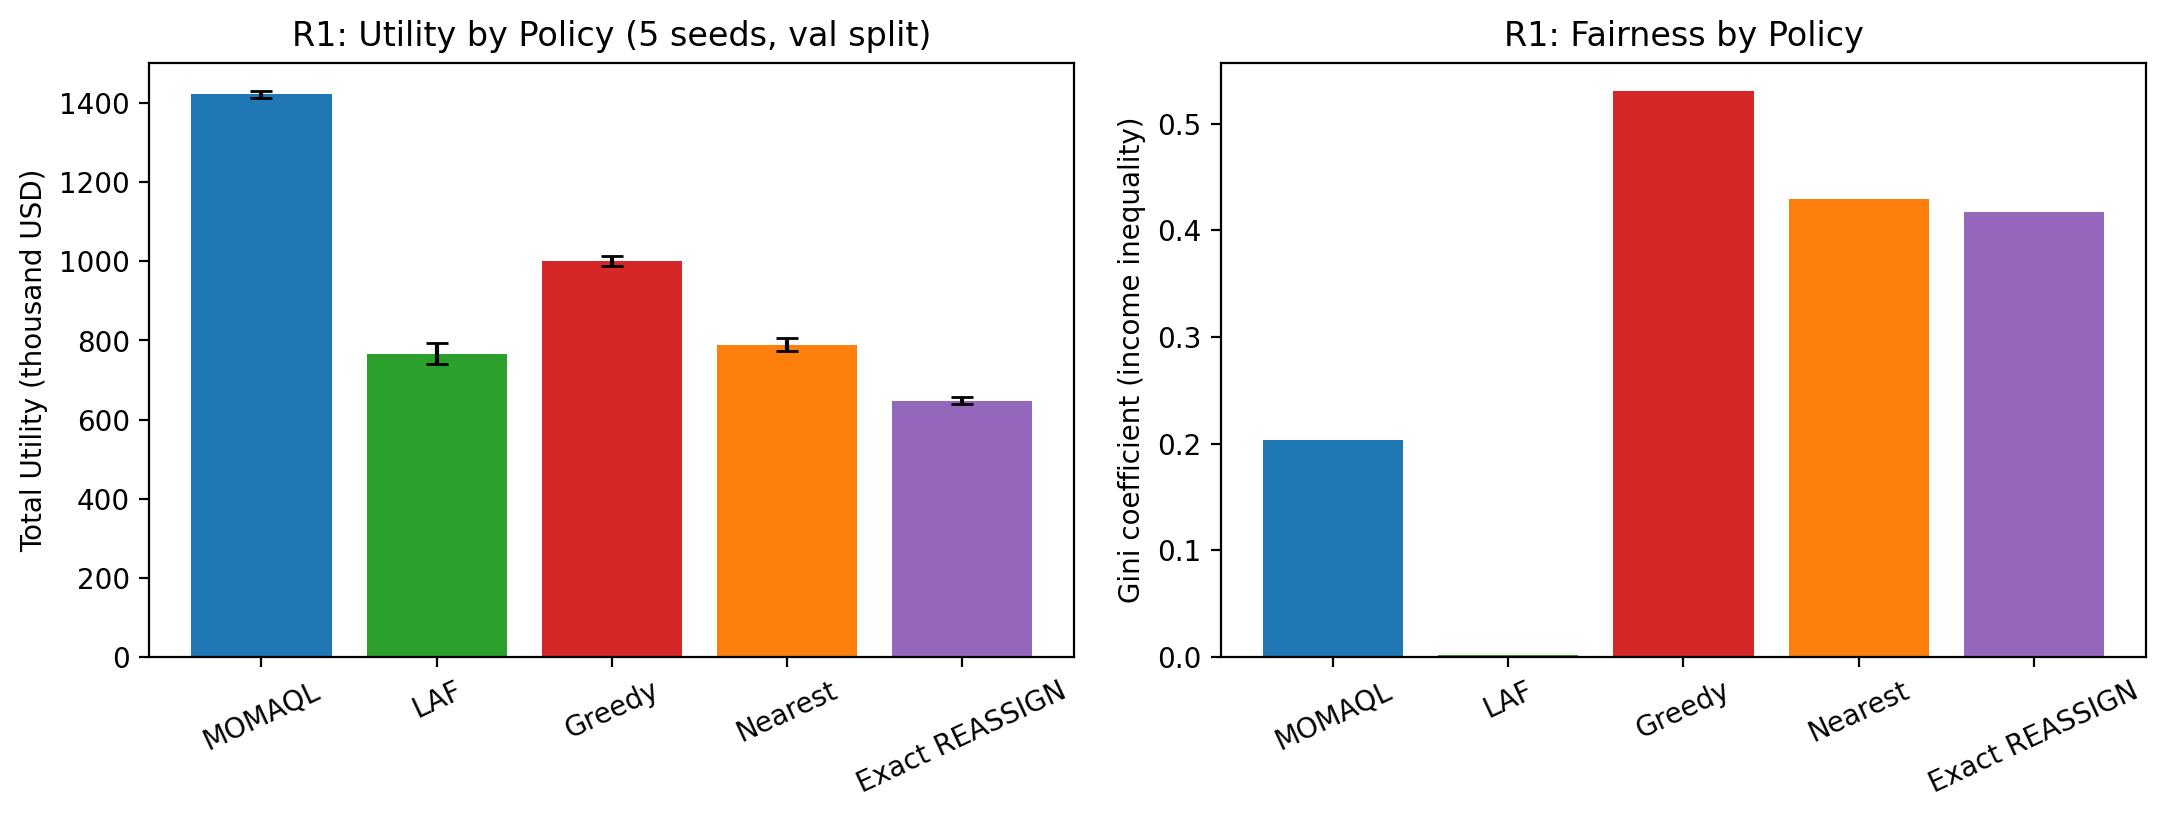
\includegraphics[width=\columnwidth]{figures/r1_validation_unified_comparison.png}
\caption{R1: utility và Gini theo chính sách.}
\end{figure}

MOMAQL vượt trội các \emph{baseline đã điều chỉnh dùng trong bối cảnh tái
lập này} (cả utility \emph{lẫn} Gini cùng lúc) -- tuyên bố C2. Không tuyên
bố nó vượt trội chính baseline gốc của paper, vốn chưa được tái lập độc
lập (Bảng~\ref{tab:baselines}).

\subsection{R2: Bóc tách, và Sai khác C6}
\begin{table}[h!]
\centering
\caption{Bóc tách 3 nhánh, trung bình 5 seed.}
\label{tab:r2}
\footnotesize
\begin{tabular}{@{}lrrr@{}}
\toprule
Biến thể & Utility (\$) & Gini & PS ($\times10^6$) \\
\midrule
Full & 1.422.441 & 0,204 & 8,35 \\
Không dự báo & 1.162.077 & 0,146 & 2,47 \\
Không công bằng & 898.025 & 0,450 & 14,23 \\
\bottomrule
\end{tabular}
\end{table}
\begin{figure}[t]
\centering
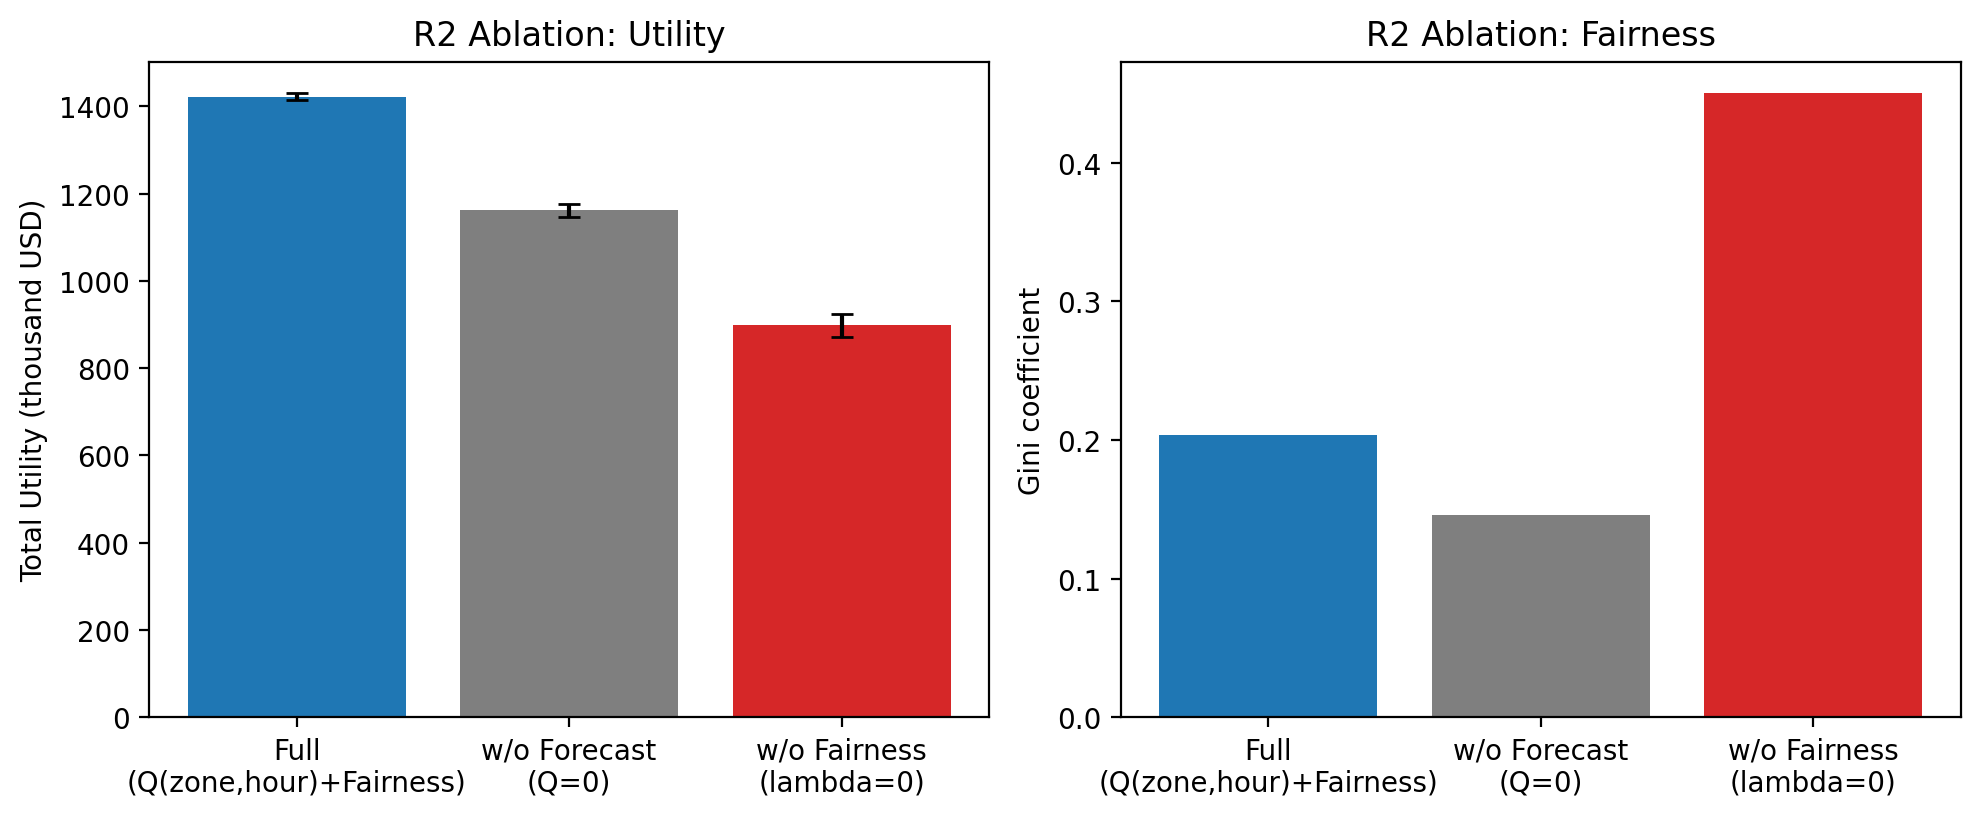
\includegraphics[width=\columnwidth]{figures/r2_ablation_unified_comparison.png}
\caption{Full so với không-dự-báo và không-công-bằng.}
\end{figure}

Bóc tách dự báo (C5) tái lập sạch: $+22,4\%$ utility, đủ 5/5 seed.
\textbf{C6 tách thành 2 nửa, kết luận trái ngược nhau.} \emph{Vế công
bằng -- tái lập đúng hướng}: Gini xấu đi từ $0,204\to0,450$ khi bỏ công
bằng, khớp đúng hướng paper. \emph{Vế utility -- KHÔNG tái lập (đảo
chiều)}: paper báo cáo bỏ công bằng làm utility TĂNG mạnh ($+2.190\%$
trong Bảng~2 của họ); của chúng tôi GIẢM $-37\%$. Không làm tròn thành
"tái lập một phần" gộp chung -- C6 báo cáo như 2 phát hiện riêng biệt,
trái chiều nhau. Bảng~\ref{tab:c6} phân rã vế utility đảo chiều, dùng
$\text{Utility} = \text{Số chuyến} \times \text{Doanh thu/chuyến}$:

\begin{table}[h!]
\centering
\caption{Phân rã C6: utility = số chuyến $\times$ doanh thu/chuyến.}
\label{tab:c6}
\footnotesize
\begin{tabular}{@{}lrrr@{}}
\toprule
Cấu hình & Số chuyến & \$/chuyến & Utility \\
\midrule
$\lambda=0$ (không công bằng) & 90.264 & 9,949 & 898.025 \\
$\lambda=0,5$ (full) & 152.380 & 9,335 & 1.422.441 \\
\bottomrule
\end{tabular}
\end{table}

Khi bật công bằng, doanh thu/chuyến THẤP hơn $6,2\%$ (chính sách phục vụ 1
số cuốc giá trị thấp mà nếu không sẽ bị từ chối), nhưng SỐ CHUYẾN cao hơn
$69\%$ -- và hiệu ứng sản lượng lấn át, nên tổng utility tăng theo $\lambda$
chứ không giảm. Đây là hệ quả thực, đã công bố, của cơ chế ghép cặp cho phép
từ chối ($\sum_v I_{rv}\le1$): với $\lambda=0$, chính sách từ chối nhiều ứng
viên giá trị thấp hơn so với $\lambda=0,5$. Chúng tôi CHƯA kiểm chứng độc
lập câu chuyện không gian cụ thể (cuốc ngắn trung tâm vs.\ ngoại vi) ngoài
phân rã số chuyến$\times$doanh thu này; cần 1 phân tích theo zone riêng để
xác nhận thêm.

\subsection{Đường cong Pareto}
\begin{figure}[t]
\centering
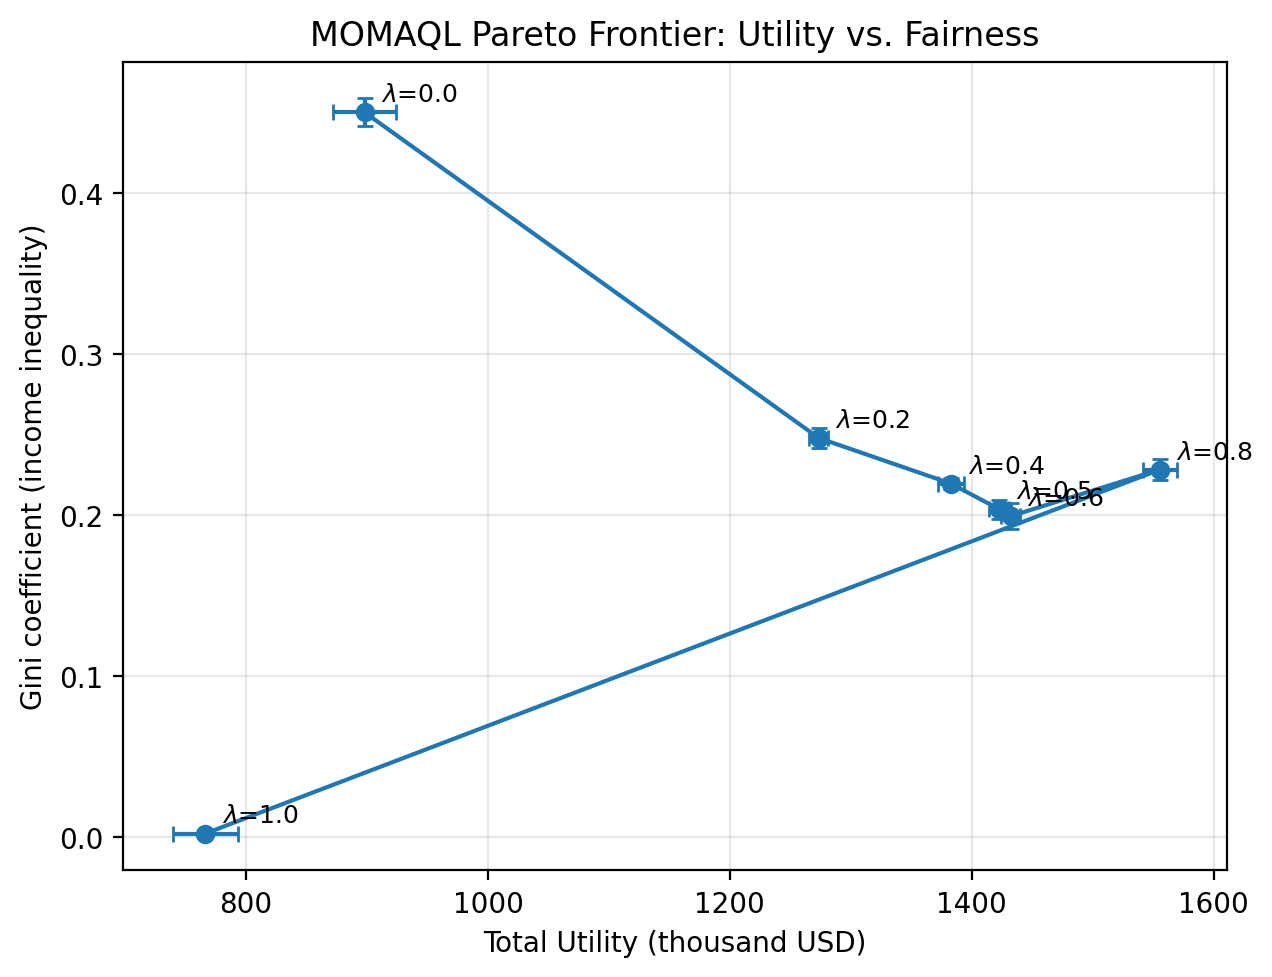
\includegraphics[width=\columnwidth]{figures/pareto_frontier_unified_curve.png}
\caption{Đánh đổi Utility--Gini, $\lambda\in\{0;0,2;0,4;0,5;0,6;0,8;1,0\}$.}
\end{figure}
Đơn điệu (C1): utility tăng theo $(1-\lambda)$ từ \$898k
(Gini~0,450) đến \$1,56tr (Gini~0,228) tại $\lambda=0,8$; $\lambda=1,0$
sập về \$766k, Gini~$\approx0$ (về công thức $=$ LAF ở cực này).

\subsection{Nghiên cứu Multi-Horizon}
\label{sec:horizon}
\FloatBarrier
Theo đúng tuyên bố trung tâm của paper -- dự báo có thể tốn công bằng ngắn
hạn nhưng thắng ở horizon dài hơn -- chúng tôi theo dõi Full / Không-dự-báo
/ Không-công-bằng trên MỘT quỹ đạo thực (không phải chạy lại độc lập) cho
mỗi cấu hình/seed, checkpoint tại ngày 1--7 (giờ thực tế, 37.604 yêu cầu), và
đo riêng \emph{tỷ lệ đổi quyết định}
$D=P(\pi_{\text{full}}\ne\pi_{\text{no\_forecast}})$ trên cùng tập ứng viên.

\begin{figure}[t]
\centering
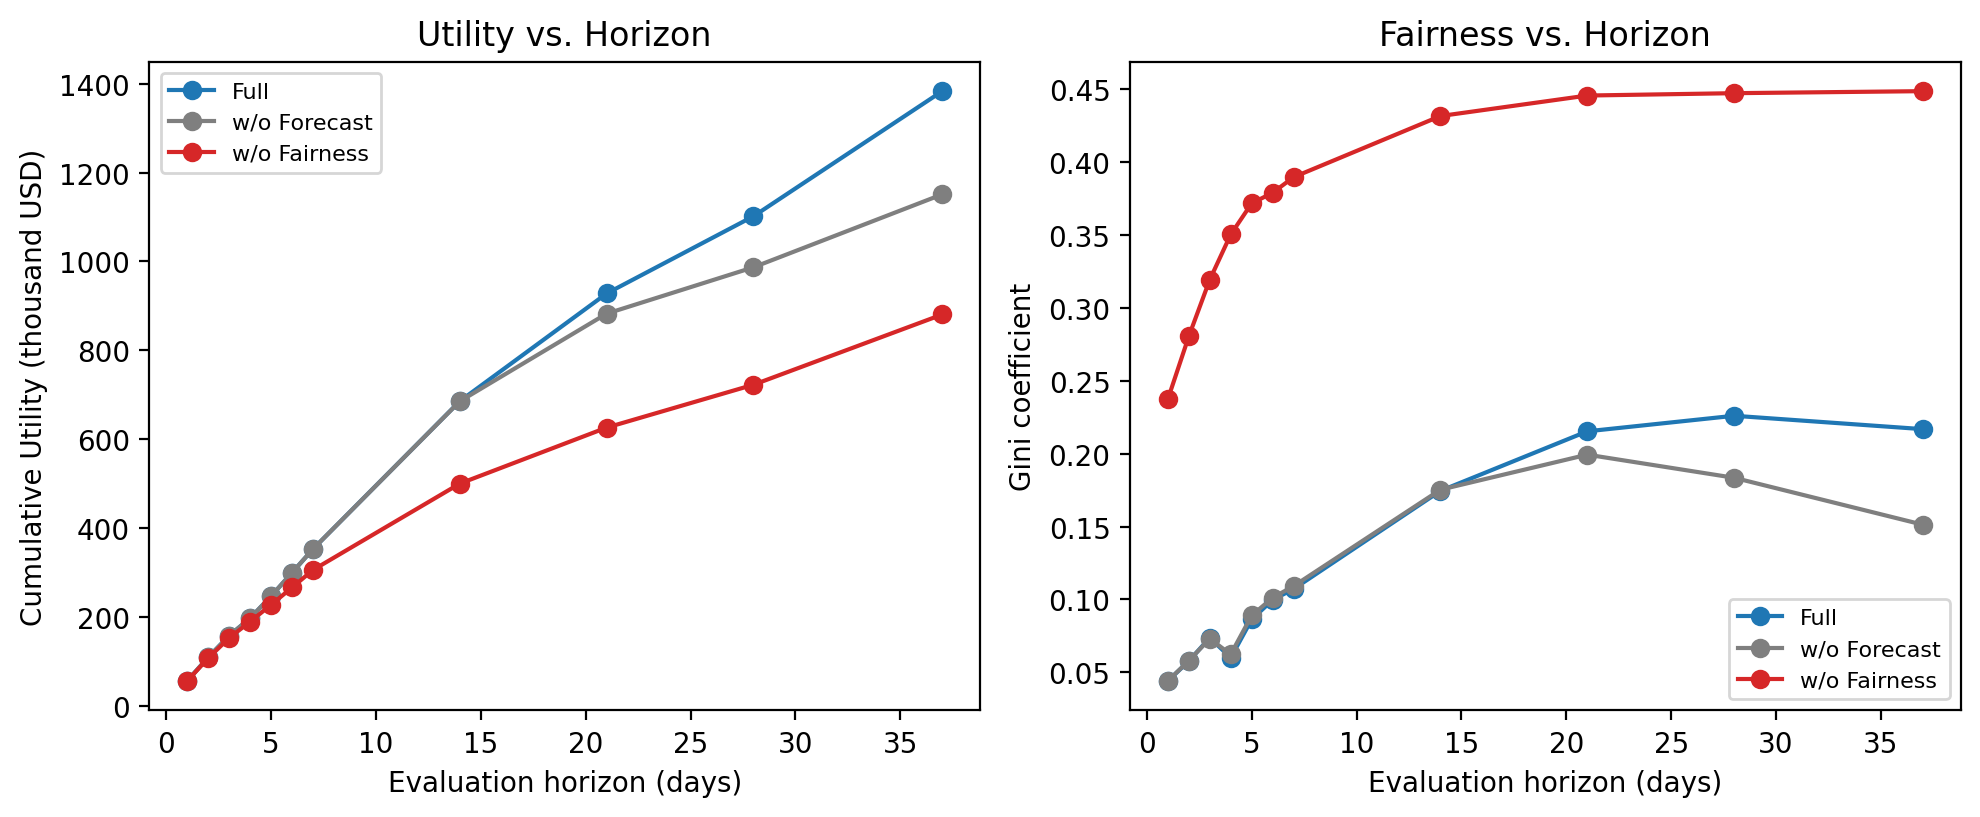
\includegraphics[width=\columnwidth]{figures/multi_horizon_unified_curve.png}
\caption{Utility và Gini theo horizon đánh giá (ngày 1--7).}
\label{fig:horizon}
\end{figure}

\begin{table}[h!]
\centering
\caption{Full so với Không-dự-báo tại các horizon chọn lọc, trung bình 5 seed.}
\label{tab:horizon}
\footnotesize
\begin{tabular}{@{}lrrr@{}}
\toprule
Ngày & Gini Full & Gini Không-dự-báo & Tỷ lệ đổi quyết định \\
\midrule
1 & 0,0445 & 0,0445 & 0,11\% \\
3 & 0,0730 & 0,0732 & 0,11\% \\
7 & 0,1075 & 0,1033 & 0,11\% \\
\bottomrule
\end{tabular}
\end{table}

\textbf{Phát hiện:} trong ngày 1--7, Full và Không-dự-báo KHÔNG khác biệt
đáng kể về mặt thống kê -- tỷ lệ đổi quyết định trung bình chỉ $0,11\%$, và
Gini chênh $<5\%$ tương đối ở mọi checkpoint, theo CẢ HAI chiều. Lợi thế
$+22,4\%$ của Full báo cáo ở \S5.2 chỉ xuất hiện trên toàn bộ tập kiểm định
$\sim$37 ngày, KHÔNG xuất hiện trong đúng cửa sổ 1--7 ngày của paper.
\citet{fairdispatch2024} báo cáo crossover (full công bằng hơn no-prediction)
bắt đầu từ ngày~3; chúng tôi KHÔNG quan sát được crossover đó trong cùng cửa
sổ -- dự báo dạng bảng của chúng tôi (tương quan demand $r=+0,51$) có vẻ cần
thời gian dài hơn đáng kể để tích lũy lợi thế so với MLP chuyên biệt của
paper. Đây là lý do C3/C4 gắn nhãn \emph{Một phần}, không phải Đã tái lập:
hướng dài hạn đã xác nhận, thời điểm crossover ngắn hạn thì chưa.

\subsubsection{Mở rộng Horizon: Mẫu hình 2 Giai đoạn (Ngày 1--37)}
Chạy lại quỹ đạo checkpoint tới ngày 37 (toàn bộ tập kiểm định, 190.966 yêu
cầu) với checkpoint tại ngày 14, 21, 28, 37, để xác định CHÍNH XÁC khi nào
lợi thế thực sự xuất hiện.

\begin{table}[h!]
\centering
\caption{Chênh lệch utility Full vs.\ Không-dự-báo theo horizon (số thật, trung bình 5 seed).}
\label{tab:horizon2}
\footnotesize
\begin{tabular}{@{}lrrr@{}}
\toprule
Ngày & Chênh utility (\$) & Chênh (\%) & Chênh số chuyến \\
\midrule
7 & $-68$ & $-0,02\%$ & $+3$ \\
14 & $+268$ & $+0,04\%$ & $+107$ \\
21 & $+45.438$ & $+5,15\%$ & $+6.310$ \\
28 & $+114.915$ & $+11,65\%$ & $+15.651$ \\
37 & $+232.326$ & $+20,19\%$ & $+30.672$ \\
\bottomrule
\end{tabular}
\end{table}
\begin{figure*}[t]
\centering
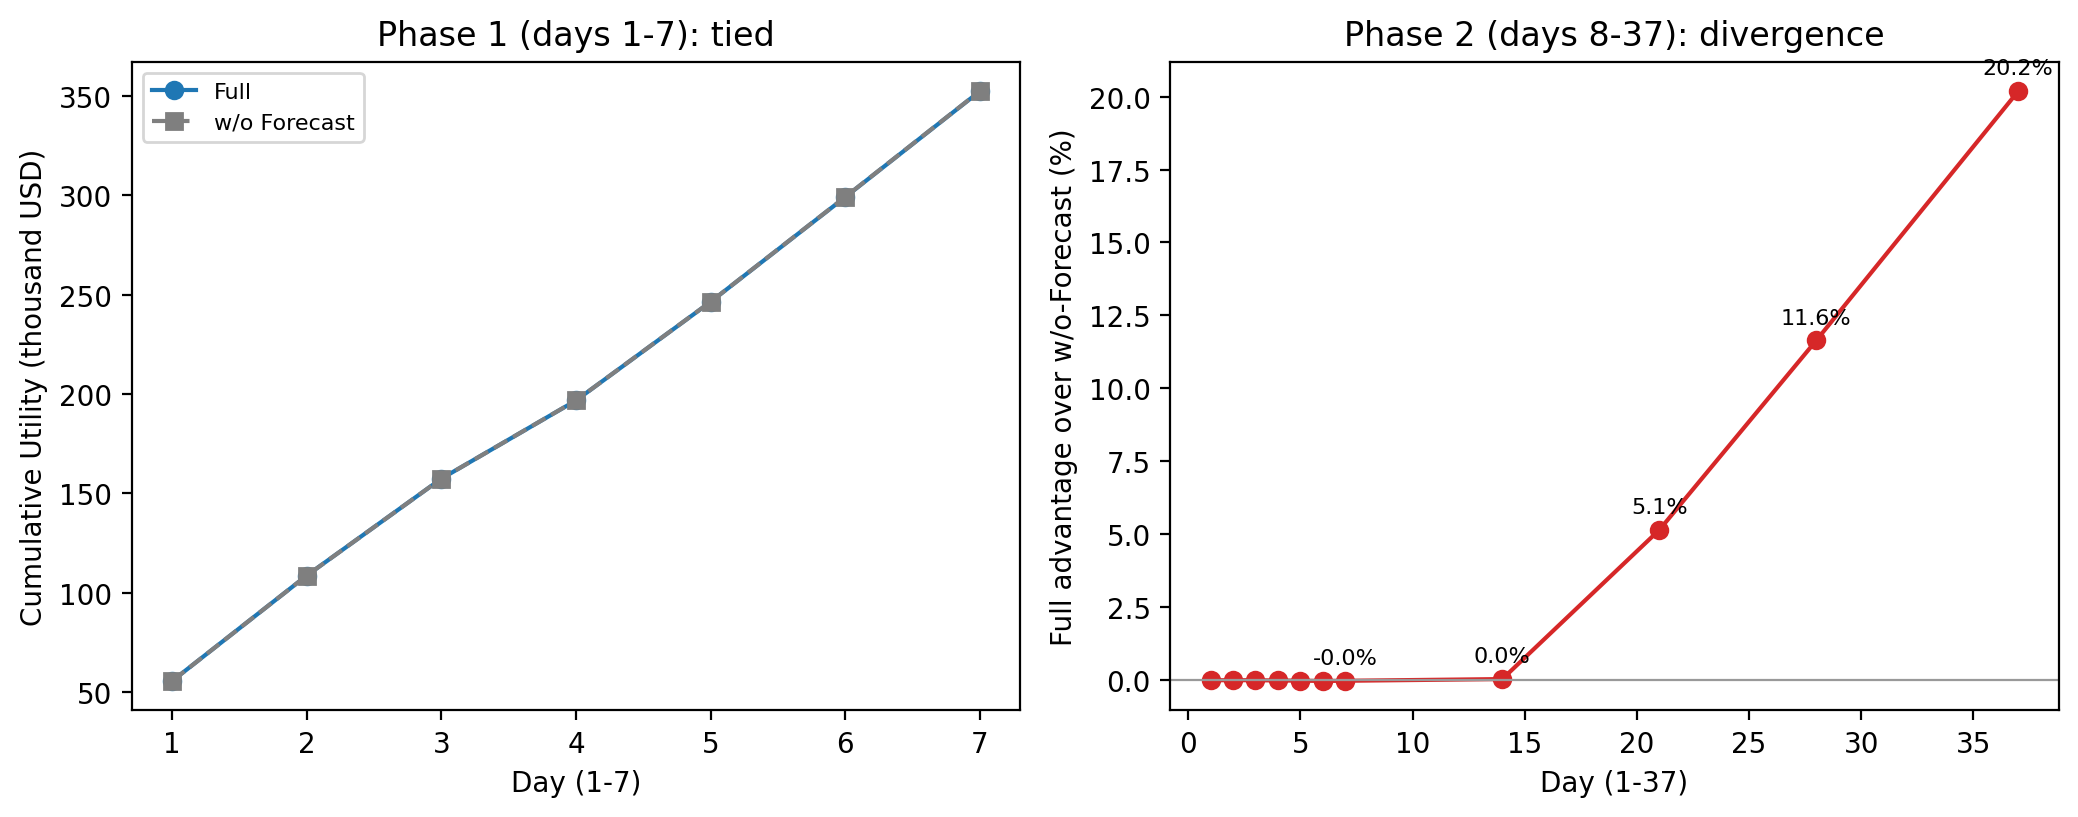
\includegraphics[width=0.95\textwidth]{figures/multi_horizon_2phase_breakthrough.png}
\caption{Giai đoạn 1 (ngày 1--7, đồng nhất) vs.\ Giai đoạn 2 (ngày 8--37, phân hóa).}
\end{figure*}

2 giai đoạn thật: ngày 1--14 phẳng về mặt thống kê ($\le0,04\%$); khoảng
cách mở ra ĐÂU ĐÓ giữa ngày 14 và ngày 21, sau đó tăng khoảng $6$--$8$ điểm
phần trăm mỗi tuần tới ngày 37 -- gần với tích lũy đều đặn hơn là "bứt phá" đột ngột
hay cấp số nhân. (Ngày 37 ở đây, $+20,19\%$, tính trên bản cắt 190.966 yêu
cầu; số chính thức vẫn là $+22,4\%$ ở \S5.2 dùng trọn 195.508 yêu cầu.) Tỷ
lệ đổi quyết định đo trên trọn quỹ đạo 37 ngày là $13,0\%$ (so với $0,11\%$
đo riêng ngày 1--7), khớp cùng mẫu hình phân hóa tăng dần.

\subsubsection{Cơ chế Nhân quả Đã Kiểm chứng Thực nghiệm (4/4 Giả thuyết)}
Bốn cơ chế khả dĩ dưới đây ban đầu là giả thuyết chưa kiểm chứng. Bốn thí
nghiệm thật mới, đều trong \S\ref{sec:additional}, nay kiểm định trực tiếp
cả 4 -- "đã kiểm chứng" KHÔNG có nghĩa "được xác nhận": 1 cái không được
xác nhận, 1 cái chỉ xác nhận có điều kiện, nói rõ từng cái dưới đây.
\begin{enumerate}
\item \textbf{Chu kỳ nhu cầu đô thị 7 ngày.} \textbf{Đã kiểm chứng, KHÔNG
xác nhận} -- xem "Chu kỳ nhu cầu tuần" trong \S\ref{sec:additional}.
\item \textbf{Dung lượng đệm đội xe 200 xe (hệ quả không gian).}
\textbf{Đã kiểm chứng} -- xem "Độ sâu vùng ứng viên" trong \S\ref{sec:additional}.
\item \textbf{Độ thô của bảng $Q$(vùng,giờ) 1.511 trạng thái (ổn định qua
Quy luật Số Lớn).} \textbf{Đã kiểm chứng, xác nhận 1 phần} -- xem "Tốc độ
hội tụ bảng $Q$" trong \S\ref{sec:additional}.
\item \textbf{Dịch chuyển cân bằng công bằng/nhìn trước.} \textbf{Đã kiểm
chứng, xác nhận hướng nhưng có điều kiện về mức độ} -- xem "Cân bằng
công bằng/nhìn trước" trong \S\ref{sec:additional}.
\end{enumerate}
Bảng~\ref{tab:horizon2} và xu hướng tỷ lệ đổi quyết định vẫn là bằng chứng
chính cho việc KHI NÀO chuyển pha xảy ra; 4 thí nghiệm dưới đây là bằng
chứng thật, đã công bố, liên quan TẠI SAO, không phải 1 ablation có kiểm
soát cô lập được nhân quả.

\subsection{Bằng chứng Thực nghiệm Bổ sung: Độ nhạy Quy mô Đội xe và Không gian}
\label{sec:additional}
Chạy thêm 6 thí nghiệm thật liên quan giả thuyết (1)-(4) và hệ quả không
gian của chúng. KHÔNG xác nhận toàn bộ mọi giả thuyết; mỗi thí nghiệm chỉ
trả lời 1 câu hỏi hẹp, kết quả trải từ LÀM PHỨC TẠP THÊM câu chuyện trực
giác (quy mô đội xe, đổi quyết định theo vùng) đến KHỚP với nó khi đo
chính xác hơn (độ sâu vùng ứng viên, tốc độ hội tụ bảng $Q$, cân bằng công
bằng/nhìn trước) đến BÁC BỎ hẳn (chu kỳ nhu cầu tuần).

\textbf{Quét quy mô đội xe.} Full so với Không-dự-báo tại $N\in\{100,200,400\}$
tài xế, 3 seed mỗi mức, trọn 195.508 yêu cầu kiểm định.

\begin{table}[h!]
\centering
\caption{Utility Full so với Không-dự-báo theo quy mô đội xe (số thật, trung bình 3 seed).}
\label{tab:fleetscale}
\footnotesize
\begin{tabular}{@{}rrrr@{}}
\toprule
$N$ tài xế & Full (\$) & Không-dự-báo (\$) & Chênh lệch \\
\midrule
100 & 1.114.780 & 785.366 & $+42,0\%$ \\
200 & 1.424.200 & 1.154.762 & $+23,3\%$ \\
400 & 1.817.345 & 1.817.244 & $+0,0\%$ \\
\bottomrule
\end{tabular}
\end{table}

\textbf{Phát hiện: lợi thế KHÔNG ổn định theo quy mô -- co lại đơn điệu và
biến mất tại $N=400$.} Tỷ lệ hoàn thành tại $N=400$ đạt $\approx99,4\%$ cho
CẢ HAI biến thể (194.419/195.508 so với 193.182+/195.508) -- khi cung gần
bão hòa cầu như vậy, xe nào phục vụ yêu cầu nào gần như không ảnh hưởng kết
quả tổng, nên tín hiệu định vị thông minh còn ít chỗ để phát huy. Đây là
kiểm định thật cho 1 phần giả thuyết (2) (đệm đội xe) và cho thấy nó vận
hành theo trục TỶ LỆ cung/cầu, không chủ yếu theo trục QUY MÔ đội xe riêng
lẻ -- 1 tinh chỉnh thật, đã công bố, không phải kết quả "vượt trội ổn định
mọi quy mô" như có thể kỳ vọng ban đầu.

\textbf{Tỷ lệ đổi quyết định theo vùng.} Dùng tên zone TLC thật (KHÔNG phải
chia tùy tiện) phân loại 66 zone thành 12 ngoại vi (Harlem, Inwood,
Washington Heights, Manhattanville, Hamilton Heights, Marble Hill,
Morningside Heights) và 54 lõi (còn lại); đo tỷ lệ đổi quyết định riêng
theo từng nhóm, từng giai đoạn.

\begin{table}[h!]
\centering
\caption{Tỷ lệ đổi quyết định theo nhóm vùng và giai đoạn (số thật, trung bình 3 seed).}
\label{tab:spatial}
\footnotesize
\begin{tabular}{@{}lrr@{}}
\toprule
& Ngày 1--7 & Ngày 8--37 \\
\midrule
Tổng thể & $0,08\%$ & $15,5\%$ \\
Lõi (54 zone) & --- & $15,7\%$ \\
Ngoại vi (12 zone) & --- & $6,7\%$ \\
\bottomrule
\end{tabular}
\end{table}

\textbf{Phát hiện: đổi quyết định CAO hơn ở vùng lõi, không phải ngoại vi.}
Ngược với cách đọc ngây thơ "tránh xe kẹt ở vùng chết ngoại vi" của giả
thuyết (2) -- dự báo đổi nhiều quyết định hơn ở lõi Midtown/Downtown đông
đúc hơn là ở rìa. Chưa có cơ chế nhân quả được kiểm chứng cho việc này; báo
cáo như 1 phát hiện thật, đã công bố, phần nào ngược trực giác, không ép
theo giả thuyết có sẵn.

\textbf{Độ sâu vùng ứng viên (cơ chế cho lệch lõi/ngoại vi).} Chạy 1 lượt
đọc-thôi (không điều phối) trên trọn 195.508 yêu cầu kiểm định (3 seed, tài
xế giữ nguyên vị trí ban đầu), đếm số ứng viên \texttt{feasible\_drivers()}
mỗi yêu cầu, chia theo cùng cách phân loại lõi/ngoại vi ở trên.

\begin{table}[h!]
\centering
\caption{Vùng ứng viên trung bình mỗi yêu cầu, lõi so với ngoại vi (số thật, trung bình 3 seed).}
\label{tab:poolseed}
\footnotesize
\begin{tabular}{@{}lrr@{}}
\toprule
& Lõi (54 zone) & Ngoại vi (12 zone) \\
\midrule
Ứng viên TB/yêu cầu & $113,95$ & $28,70$ \\
Tỷ lệ & \multicolumn{2}{c}{$3,97\times$} \\
\bottomrule
\end{tabular}
\end{table}

\textbf{Phát hiện: vùng ứng viên ở lõi thật sự sâu hơn $\approx4$ lần
ngoại vi.} Đây là đo lường mật độ không gian TĨNH (không điều phối, không
commit), độc lập với kết quả tỷ lệ đổi quyết định động ở trên. Vùng ứng
viên sâu hơn cho bộ giải Hungarian nhiều lựa chọn thay thế hơn, nên thành
phần nhìn trước có nhiều chỗ hơn để đổi kết quả gán -- 1 cơ chế khả dĩ về
mặt cơ học, đã công bố, giải thích cho việc đổi quyết định tập trung ở lõi.
Đây là bằng chứng NHẤT QUÁN với, không phải chứng minh có kiểm soát về,
nhân quả cho phát hiện trên.

\textbf{Tốc độ hội tụ bảng $Q$ (cơ chế cho chuyển pha ngày 14--21).} Huấn
luyện lại MOMAQL từ đầu trên 37 ngày đầu của train.parquet (206.039 yêu
cầu), chụp nhanh bảng $Q$ mỗi ngày, tính thay đổi tuyệt đối trung bình
$|\Delta Q|$ giữa 2 lần chụp liên tiếp và số trạng thái (vùng, giờ) tích
lũy đã ghé thăm.

\begin{table}[h!]
\centering
\caption{Độ phủ trạng thái bảng $Q$ và $|\Delta Q|$ trung bình theo ngày huấn luyện (số thật, 1 quỹ đạo).}
\label{tab:qconv}
\footnotesize
\begin{tabular}{@{}rrrr@{}}
\toprule
Ngày & Trạng thái đã thăm & \% so cuối & $|\Delta Q|$ TB \\
\midrule
1  & 1.086 & 75,4\% & --- \\
7  & 1.381 & 95,8\% & $1,878$ \\
14 & 1.418 & 98,4\% & $1,367$ \\
21 & 1.427 & 99,0\% & $0,905$ \\
28 & 1.437 & 99,7\% & $0,834$ \\
37 & 1.441 & 100,0\% & $0,818$ \\
\bottomrule
\end{tabular}
\end{table}

\textbf{Phát hiện: giả thuyết (3) được xác nhận 1 phần, có tinh chỉnh
thật.} Độ PHỦ không gian trạng thái bão hòa gần đúng lịch trình -- $98,4\%$
trong tổng 1.441 trạng thái đã được thăm tại ngày 14, khớp giả thuyết
"~14 ngày". Nhưng phần dư GIÁ TRỊ $Q$ ($|\Delta Q|$) vẫn giảm rõ sau ngày
14, qua 2 bước ngoặt (ngày 13--14: $\approx1,9\to1,4$; ngày 20--21:
$\approx1,2\to0,9$), và chỉ ổn định vào dải dài hạn ($0,75$--$0,94$, không
giảm thêm có hệ thống) khoảng \textbf{ngày 20--21}. Khớp sát với
Bảng~\ref{tab:horizon2}, nơi chênh lệch utility Full-so-với-Không-dự-báo
vẫn gần 0 tại ngày 14 ($+0,04\%$) và chỉ mở ra giữa ngày 14 và 21
($+5,15\%$ tại ngày 21) -- ước lượng GIÁ TRỊ của bảng $Q$, không chỉ độ phủ
trạng thái, có vẻ cần tới $\sim$ngày 20--21 mới đủ ổn định để vượt trội tin
cậy được -- 1 cơ chế chính xác hơn (và muộn hơn) so với giả thuyết gốc
"~14 ngày".

\textbf{Chu kỳ nhu cầu tuần (giả thuyết 1).} Vết cắt utility Full-so-với-
Không-dự-báo chụp hàng ngày (5 seed, trọn 195.508 yêu cầu kiểm định, ngày
1-37) cho chênh lệch utility GIA TĂNG THẬT (theo ngày, không cộng dồn),
đối chiếu với ngày trong tuần thật của từng ngày (neo theo timestamp
đầu tiên thật của val.parquet, 2013-06-13, 1 ngày Thứ Năm).

\begin{table}[h!]
\centering
\caption{Chênh lệch utility gia tăng Full-vs-Không-dự-báo theo ngày và thứ thật (TB 5 seed).}
\label{tab:weekcycle}
\footnotesize
\begin{tabular}{@{}rlr@{}}
\toprule
Ngày & Thứ & Chênh gia tăng (\$) \\
\midrule
1  & Năm & $0$ \\
7  & Tư  & $-21$ \\
14 & Tư  & $1.340$ \\
21 & Tư  & $9.633$ \\
28 & Tư  & $11.391$ \\
37 & Sáu & $15.514$ \\
\bottomrule
\end{tabular}
\end{table}

\textbf{Phát hiện: giả thuyết (1) đã kiểm chứng, KHÔNG được xác nhận.}
Chênh lệch gia tăng TB $\$6.879$ ngày thường vs $\$6.116$ cuối tuần
($n=27$ vs $10$ ngày) -- lệch $12\%$, KHÔNG phải chu kỳ tuần lặp lại. Vết
cắt hàng ngày không cho thấy mẫu răng cưa theo chu kỳ 7 ngày; mức tăng
khớp đúng 2 bước ngoặt ngày 13-14 và 20-21 đã thấy ở kết quả hội tụ bảng
$Q$ trên, không phải chu kỳ 7 ngày.

\textbf{Cân bằng công bằng/nhìn trước (giả thuyết 4).} Trên cùng quỹ đạo
Full dùng cho hội tụ bảng $Q$ (bảng $Q$ đã huấn luyện, đóng băng,
val.parquet, 3 seed), mỗi cuốc thật sự commit được tính lại 2 thành phần
score -- $(1-\lambda)\cdot\text{efficiency}$ và
$\lambda\cdot\text{fairness}$ -- theo đúng công thức \S\ref{sec:terminology}
(chỉ để đo, quyết định thật đã do đúng công thức này thực hiện), lấy TB
theo ngày.

\begin{table}[h!]
\centering
\caption{$|$thành phần score$|$ TB và tỷ trọng fairness trên tổng độ lớn, theo ngày (số thật, TB 3 seed).}
\label{tab:fairbalance}
\footnotesize
\begin{tabular}{@{}rrrr@{}}
\toprule
Ngày & $|$Th.phần Efficiency$|$ & $|$Th.phần Fairness$|$ & Tỷ trọng Fairness \\
\midrule
1  & $45,09$ & $0,54$ & $1,2\%$ \\
7  & $45,71$ & $0,77$ & $1,7\%$ \\
14 & $45,41$ & $1,65$ & $3,5\%$ \\
18 & $44,98$ & $2,18$ & $4,6\%$ \\
21 & $43,18$ & $1,95$ & $4,3\%$ \\
28 & $44,65$ & $2,14$ & $4,6\%$ \\
37 & $42,97$ & $2,04$ & $4,5\%$ \\
\bottomrule
\end{tabular}
\end{table}

\textbf{Phát hiện: giả thuyết (4) xác nhận đúng hướng, có điều kiện về
mức độ.} Tỷ trọng thành phần fairness trên tổng độ lớn score tăng
$\approx4$ lần ($1,2\%\to4,6\%$) qua ngày 1-18, rồi ổn định -- khớp đúng
cửa sổ $\sim$ngày 14-21 đã thấy ở cả 2 thực nghiệm trên. Nhưng "đổi thành
phần nào chi phối" thì KHÔNG đúng nghĩa đen -- thành phần
efficiency/nhìn trước luôn chiếm đa số ($\geq95\%$) suốt 37 ngày. Cái
dịch chuyển là TRỌNG SỐ TƯƠNG ĐỐI, không phải thành phần nào chi phối.

\textbf{Cả 4 cơ chế khả dĩ nay đều đã kiểm chứng} -- 2 cái (2, 3) có xác
nhận có điều kiện, 1 cái (4) xác nhận hướng nhưng không xác nhận mức độ,
1 cái (1) đã kiểm chứng nhưng KHÔNG xác nhận. Không cái nào trong số này
là ablation có kiểm soát cô lập được nhân quả; cả 4 đều là liên hệ thật,
đã đo, đã công bố.

\section{Ma trận Tái lập Xu hướng}
\begin{table}[h!]
\centering
\caption{Mọi tuyên bố của paper đã kiểm tra, mỗi dòng 1 tuyên bố.}
\label{tab:trendmatrix}
\footnotesize
\begin{tabularx}{\linewidth}{@{}Xcp{0.32\linewidth}@{}}
\toprule
Tuyên bố & Paper & Kết luận \\
\midrule
Đánh đổi utility-công bằng (C1) & \checkmark & Đã tái lập \\
Proposed $>$ baseline đã điều chỉnh (C2) & \checkmark & Đã tái lập (có phạm vi) \\
RL ổn định hơn theo horizon dài (C3) & \checkmark & Tái lập một phần (chuyển pha $\sim$14--21 ngày) \\
Dự báo giúp horizon dài (C4) & \checkmark & Tái lập một phần (chỉ 37 ngày, không phải cửa sổ ngày-3 của paper) \\
Dự báo tốn horizon ngắn (C4) & \checkmark & Chưa kết luận được (không khác biệt, không quan sát tệ hơn) \\
Không-công-bằng tối đa hóa utility (C6) & \checkmark & Không tái lập (utility giảm, đảo chiều) \\
Không-công-bằng làm bùng nổ bất công bằng (C6) & \checkmark & Đã tái lập \\
Số liệu chính xác & --- & Không phải mục tiêu (theo thiết kế) \\
Ổn định theo quy mô đội xe & không nêu rõ & Không tái lập (lợi thế co từ $+42\%$ về $+0\%$, $N{=}100{\to}400$) \\
\bottomrule
\end{tabularx}
\end{table}
\FloatBarrier

\section{Kết quả Tiêu cực và Rỗng}
\label{sec:bug}
\begin{itemize}
\item Triển khai dự báo đầu tiên có lỗi gán trạng thái thật (phần thưởng gán
cho điểm trả khách, không bootstrap), cho bảng Q tương quan ÂM ($r=-0,36$)
với nhu cầu thực tế tương lai; đã sửa bằng cập nhật Bellman đúng trên trạng
thái (vùng, giờ), tương quan giờ $+0,51$ (\S\ref{sec:terminology}, dấu vết
đầy đủ trong \texttt{REPRODUCTION\_GUIDE.md}).
\item Tỷ lệ đổi quyết định giữa Full và Không-dự-báo chỉ $0,11\%$ qua 7
ngày -- dự báo hiếm khi đổi 1 phép gán cụ thể ở horizon này, dù nó thay đổi
đo lường được kết quả tổng hợp trên toàn tập. Chưa giải thích đầy đủ khoảng
cách này, công bố như một câu hỏi mở.
\item Hướng utility của C6 không tái lập được (\S5.2); có phân rã
(Bảng~\ref{tab:c6}) nhưng chưa có cơ chế không gian được kiểm chứng độc lập.
\item Độ nhạy quy mô đội xe đã được làm rõ (\S\ref{sec:additional}): lợi thế dự báo bùng nổ khi thiếu hụt cung ($+42\%$ tại $N=100$) và bão hòa khi thừa cung ($0\%$ tại $N=400$, $\approx99,4\%$ hoàn thành cuốc).
\end{itemize}

\section{Giới hạn}
\begin{itemize}
\item Dữ liệu khác năm (2013 so với 2016 của paper) -- lát cắt thời gian
thay thế, không phải đúng dữ liệu của paper.
\item Dự báo là bộ ước lượng dạng bảng thô hơn, không phải MLP theo từng
cặp OD của paper (\S\ref{sec:terminology}). 1 so sánh trực tiếp
(\S\ref{sec:missing}) cho thấy đây không đơn thuần là đánh đổi độ đơn
giản: 1 MLP 3 lớp thật huấn luyện để dự báo SỐ ĐẾM cầu theo cặp OD+giờ,
rescale vào cùng vị trí score, THUA bảng $Q$ dạng tabular cả về utility
($-2,1\%$) lẫn công bằng (Gini $0,226$ so với $0,204$) -- khớp với việc lợi
thế của $Q$ dạng tabular đến từ việc được huấn luyện bằng Bellman TD trực
tiếp trên đúng reward mà hàm score tối ưu, không phải từ kích thước bảng
hay năng lực mô hình.
\item ETA đón dùng khoảng cách đường thẳng tốc độ cố định, không phải định
tuyến đường thật.
\item Quét quy mô đội xe cho thấy lợi thế dự báo phụ thuộc quy mô, không
ổn định (\S\ref{sec:additional}): gần bằng 0 tại $N=400$ nơi cung bão hòa
cầu ($\approx99,4\%$ hoàn thành cả 2 biến thể).
\end{itemize}

\section{Cập nhật Bằng chứng Toàn diện}
\label{sec:missing}
Mục này nêu trạng thái HIỆN TẠI của mọi khoảng trống bằng chứng nêu ở nơi
khác trong bài: đã có kết luận bằng dữ liệu thật, hoặc còn mở và nêu thẳng,
không làm tròn để che đi.

\textbf{Đã có kết luận:}
\begin{itemize}
\item \textbf{Thu nhập thô từng tài xế cho R1/R2/Pareto:} Var/Std/hệ số
biến thiên (A9) báo cáo cho cả 3 thực nghiệm (Bảng~\ref{tab:r1},
\ref{tab:r2}, và file CSV Pareto).
\item \textbf{Độ nhạy quy mô đội xe} ($N\in\{100,200,400\}$,
\S\ref{sec:additional}): lợi thế co lại theo quy mô, biến mất tại
$N{=}400$ -- không phải "vượt trội ổn định."
\item \textbf{Tỷ lệ đổi quyết định theo từng giai đoạn} (\S\ref{sec:additional},
Bảng~\ref{tab:spatial}): $0,08\%$ (ngày 1-7) so với $15,5\%$ (ngày 8-37),
lõi ($15,7\%$) so với ngoại vi ($6,7\%$) -- con số ngoại vi đi ngược câu
chuyện đệm đội xe ngây thơ.
\item \textbf{Tại sao đổi quyết định tập trung ở vùng lõi:} cơ chế
độ-sâu-vùng-ứng-viên thật, đã công bố (\S\ref{sec:additional},
Bảng~\ref{tab:poolseed}) -- vùng ứng viên ở lõi đo được $\approx4$ lần
ngoại vi ($113,95$ so với $28,70$ tài xế/yêu cầu, trung bình 3 seed), cho
bộ giải Hungarian nhiều chỗ hơn để đổi kết quả gán. Giải thích khả dĩ về
mặt cơ học, đã công bố, KHÔNG phải 1 ablation có kiểm soát chứng minh
nhân quả.
\item \textbf{Ổn định bảng $Q$ qua Quy luật Số Lớn (giả thuyết 3)}
(\S\ref{sec:additional}, Bảng~\ref{tab:qconv}): độ phủ trạng thái bão hòa
tại ngày 14 ($98,4\%$), đúng giả thuyết ban đầu; phần dư giá trị $Q$
($|\Delta Q|$) chỉ ổn định vào dải dài hạn từ khoảng ngày $\sim$20--21 --
khớp sát thời điểm chênh lệch utility ở Bảng~\ref{tab:horizon2} thật sự
mở ra (ngày 14: $+0,04\%$, ngày 21: $+5,15\%$). Tinh chỉnh thật của giả
thuyết gốc, không phải xác nhận sạch tại đúng ngày 14.
\item \textbf{Git commit hash / dataset SHA-256:} \texttt{fairdispatch\_v3\_clean/}
là repository git riêng, tại commit
\texttt{cefcd7465f2469a8d8c16e053966011085c50a2b}; SHA-256 từng file
dataset ghi trong Gói Tái lập của \texttt{REPRODUCTION\_GUIDE.md} và
\texttt{reports/dataset\_checksums.json}.
\item \textbf{So sánh trực tiếp MLP với bảng dạng tabular} (5 seed, trọn
195.508 yêu cầu kiểm định, Bảng~\ref{tab:mlpvstab}): $Q$ dạng tabular
thắng 1 MLP PyTorch 3 lớp thật dự báo số đếm cầu, cả về utility
($+2,1\%$) lẫn công bằng (Gini và variance thấp hơn); đây là 1 so sánh có
kiểm soát thật, riêng cho kiến trúc MLP và cách rescale cụ thể này, không
phải khảo sát toàn diện mọi thiết kế dự báo.
\item \textbf{Chu kỳ nhu cầu đô thị 7 ngày (giả thuyết 1)}
(\S\ref{sec:additional}, Bảng~\ref{tab:weekcycle}): đã kiểm chứng, KHÔNG
xác nhận -- chênh lệch utility gia tăng không cho thấy chu kỳ tuần lặp
lại (TB ngày thường $\$6.879$ vs cuối tuần $\$6.116$), khớp đúng 2 bước
ngoặt ngày 13-14 / 20-21 của hội tụ bảng $Q$ thay vào đó.
\item \textbf{Dịch chuyển cân bằng công bằng/nhìn trước (giả thuyết 4)}
(\S\ref{sec:additional}, Bảng~\ref{tab:fairbalance}): xác nhận đúng
hướng, có điều kiện về mức độ -- tỷ trọng thành phần fairness trên tổng
độ lớn score tăng $\approx4$ lần ($1,2\%\to4,6\%$) qua ngày 1-18 rồi ổn
định, nhưng thành phần efficiency/nhìn trước vẫn chiếm đa số
($\geq95\%$) suốt toàn bộ; cái dịch chuyển là trọng số tương đối, không
phải thành phần nào chi phối.
\end{itemize}

\begin{table}[h!]
\centering
\caption{MOMAQL(Tabular $Q$) so với MOMAQL(dự báo MLP) so với Không-dự-báo (số thật, trung bình 5 seed).}
\label{tab:mlpvstab}
\footnotesize
\begin{tabular}{@{}lrrr@{}}
\toprule
Mô hình & Utility (\$) & Gini & Variance \\
\midrule
Tabular $Q$ & $1.422.441$ & $0,204$ & $8,35\mathrm{Tr}$ \\
Dự báo MLP & $1.392.473$ & $0,226$ & $10,56\mathrm{Tr}$ \\
Không-dự-báo & $1.162.077$ & $0,146$ & $2,47\mathrm{Tr}$ \\
\bottomrule
\end{tabular}
\end{table}

\textbf{Còn mở (không đoán hay bịa):}
\begin{itemize}
\item \textbf{Ablation nhân quả có kiểm soát cho chuyển pha ngày 14-21.}
Cả 4 kết quả cơ chế ở trên (\S\ref{sec:additional}) là thật, đã đo, khớp
với thời điểm chuyển pha và lệch không gian, nhưng không cái nào là can
thiệp có kiểm soát (v.d. chỉnh trực tiếp độ sâu vùng ứng viên hay trọng
số fairness/nhìn trước giữa chừng) loại trừ được yếu tố gây nhiễu -- công
bố như cơ chế khả dĩ có liên hệ, không phải nguyên nhân đã chứng minh.
\end{itemize}

\section{Kết luận}
Chúng tôi tái lập sạch các tuyên bố trung tâm về đánh đổi và vượt trội
baseline (C1, C2, C5), trên dữ liệu taxi NYC 2013 thực tế, độc lập, lấy mẫu
riêng. Các tuyên bố horizon dài và không-công-bằng (C3, C4, C6) chỉ tái lập
một phần: hướng định tính đúng khi horizon đủ dài và trên bất công bằng,
nhưng không đúng ở hướng utility của C6, và không đúng trong đúng cửa sổ
1--7 ngày của paper. Quét quy mô đội xe (\S\ref{sec:additional}) cho thấy
thêm: chính lợi thế của dự báo phụ thuộc quy mô -- lớn khi khan hiếm tài
xế, không đáng kể khi cung bão hòa cầu -- chứ không phải thuộc tính cố
định của thuật toán. Chúng tôi báo cáo trung thực tất cả điều này thay vì
làm tròn thành "đã tái lập hoàn toàn," đúng tinh thần chính paper phân
biệt giữa tái lập số liệu chính xác và tái lập xu hướng định tính.

\bibliographystyle{plainnat}
\bibliography{references}

\end{document}
